\section{Earth values and defects in the released codes}

An Earth value is a value or form in a model that agrees with Earth because it was set or fitted there; on
another world the model computes with it where that world's own value belongs. Such a value is a limitation
of the code, which does what it was written to do, for the world and range it was written for. A defect is
code that contradicts its own inputs, units or intent, by ignoring a configured value, restarting a clock it
should carry or reading memory never set, and it remains a defect where Earth's values or the usual
configuration make its error vanish. Earth values take four forms: constants written into the code, units
of time, geometry, and fits and simplifications used beyond their range. Three of the five defects found in
the released codes are tied to Earth's values through the same forms. Table~\ref{tab:inventory} lists the
Earth values and defects on the paths the lunar runs use, each with its form, its kind and its repair, and
the defect log in the code repository adds those found off those paths, with each one's discovery,
evidence, repair and measured effect.

\textbf{Constants written into the code.} A dimensional constant has the scale of the world it was set for,
and gravity is the commonest. CM1 release 22 sets gravity to 9.81~m\,s$^{-2}$ in four places on the lunar
cases' paths, its dynamics, the conversion of pressure to layer mass in its RRTMG radiation
\autocite{iacono2008radiative}, its CAPE diagnostic and the Morrison microphysics, as well as in schemes those
cases leave unselected, and the coefficients of Morrison's fall-speed laws $V = aD^b$ and their caps were
fitted at Earth's gravity.\claim{H01} WRF-ELEC's NSSL scheme sets 9.8 twice and ties the ventilation of
evaporating rain and depositing ice to Earth's fall-speed coefficients.\claim{H02} PlaSim diagnoses its
clouds' water with CCM3's profile \autocite{kiehl1996description}, which decays with geometric height on a
scale of $700\ln(1+\mathrm{PW})$~m written for Earth's gravity; with every pressure level six times higher,
clouds above about 20~km, most of the lunar cover, were left nearly dry.\claim{H18} WRF-ELEC's lightning
holds two thresholds and a time step set for Earth's air and storms. Its breakdown field, scaled with the
air's density \autocite{dwyer2003fundamental} and capped at 180~kV\,m$^{-1}$, meets the cap on Earth only
below about 4.5~km, beneath where flashes start, and in lunar air below about 36~km, where the cap lowers the
field by 44\% at the ground; a ground strike is declared when a channel reaches air warmer than
$-7$\,\textdegree C, about 5~km above Earth's ground and 27--34~km above the Moon's; and its 0.75~s sub-step
suits 500~m layers and Earth's fall speeds.\claim{H03} SWAN's constants come from Earth's seas. It reduces
its linear wind input above a knee fixed at 1~Hz, a value its source comments call largely arbitrary, and
because the knee stays fixed while gravity changes, stock SWAN misses a sixfold gravity-similarity test by
5.44\% in significant wave height;\claim{H04} it also fixes the air's density at 1.28~kg\,m$^{-3}$, where the
air over the lunar seas holds about 1.40.\claim{H05} Earth's composition and rotation enter the remaining
constants: RRTMG takes carbon dioxide from the calendar year and adds Earth's methane, nitrous oxide,
halocarbons and ozone, and CM1's beta plane derives its gradient from Earth's rotation and a 6,370~km
radius.\claim{H06} Options the lunar runs leave unselected, SWAN's ST6 source terms and exact nonlinear
transfer and SWASH's rotation for spherical runs, are set to Earth's gravity or rotation as well.

\textbf{Units of time.} Earth's day enters as a unit of time in the calendars and in processes that a run of
a few hours can neglect. ExoPlaSim's year of 360 days in 17,280 half-hour steps holds 12.08 lunar model days
of 1,430 steps, so output kept by model time slips 120 steps a year against the Sun.\claim{H08} CM1's Sun
follows Earth's 24-hour day, Earth's calendar and an obliquity of 23.5\textdegree, and its five soil layers,
1--16~cm thick, resolve Earth's diurnal thermal wave, which under the month-long day reaches about
0.6~m.\claim{H09} WRF-ELEC conducts no charge through clear air, its screening option acting only at cloud
edges, an omission of little weight in a storm of a few hours; in a month-long lunar run, the charge that
evaporating cloud handed to the small ions persisted for weeks and held the field at the ground near
20~kV\,m$^{-1}$ across the whole domain.\claim{H10}

\textbf{Geometry.} PlaSim and RRTMG treat each column as a stack of flat layers, lit only while the Sun
stands above that column's horizon. In the Moon's tall air the shells widen with height, sunlight crosses the
air beyond each column's horizon, and the infrared escapes through a wider top. Against the same air in flat
layers, with a pseudo-spherical direct beam for the sunlight, the curved geometry takes in 10.3~W\,m$^{-2}$
more sunlight and lets out 16.2~W\,m$^{-2}$ more infrared, a net loss of 5.8~W\,m$^{-2}$, of which the
widening of the shells accounts for 6.5 and the curved light and escape return 0.7; its twilight puts
1.4~W\,m$^{-2}$ on the ground while the Sun is below the horizon.\claim{H11} PlaSim stretches the low Sun's
water path by Earth's horizon magnification, $35/\sqrt{1+1224\mu^2}$ with $\mu$ the cosine of the solar
zenith angle \autocite{lacis1974parameterization,rodgers1967use}, where the Moon's factor is 13.5 for water
vapour and 7.1 for well-mixed air (Figure~\ref{fig:slant}).\claim{H12} The dynamics hold the same flat or
thin geometry: PlaSim's treat the air as a thin shell and CM1's as a flat slab, both with gravity constant
with height, while the in-house reference models take $g = GM/r^2$, and lunar gravity falls 5.4\% by the
air's mass-mean height and 15.3\% by CM1's 150~km top.\claim{H13} PlaSim's ten $\sigma$ levels sit at
fractions of the surface pressure chosen for Earth's air. On the Moon they put the top three layers above
107~km, at 81--107~km and at 63--81~km, each spanning about 25~K, with ice saturation changing 55-fold across
the second, and leave two layers for the lowest 6.5~km, too few to resolve the boundary layer's day--night
shape.\claim{H33}

\textbf{Fits and simplifications beyond their range.} The radiation schemes were fitted to Earth's columns
and Earth's Sun, and the lunar columns lie far outside both. PlaSim's near-infrared water absorptivity,
Lacis and Hansen's fit to Earth's water paths \autocite{lacis1974parameterization}, levels off toward half
the sunlight, and over the Moon's longer paths it left the air absorbing 7.7--8.2 points too little of the
arriving sunlight on eleven columns.\claim{H14} ExoPlaSim normalises its Rayleigh coefficient to the
ultraviolet of a 5772~K blackbody, which for the shield-filtered Sun gives a coefficient too low, and
PlaSim's water continuum over-absorbs at lunar paths; uncalibrated, the first design run, with 25\% seas
under the undimmed shield, passed 310~K and was still warming at 315.5~K in model year 12.\claim{H15}
PlaSim's two shortwave bands omit carbon dioxide and oxygen, whose lines absorb sunlight high in a column
7.25 times Earth's, so a water multiplier calibrated on the column's total put their share of the
absorption lower down, where the water is.\claim{H16} PlaSim's longwave, Sasamori's broadband
absorptivities \autocite{sasamori1968radiative} with a water continuum that the first calibration fitted to
the outgoing flux, leaves the cooling by height unconstrained: against the correlated-$k$ reference it cools
the lowest two layers by 9.7--11.9~W\,m$^{-2}$ too much and the air aloft by up to 12~W\,m$^{-2}$ too
little.\claim{H17} It gives every cloud the optics of liquid water and reckons saturation over liquid at
every temperature, so the high cloud in its second layer from the top, at 180--204~K, forms only at
136--149\% of ice saturation.\claim{H19} In CM1, RRTMG's reference pressures begin at 1,053.63~hPa, and the
lowest 7.5~km of air over the lunar sea, at up to 1,216~hPa, lie beyond them and are extrapolated in $\ln p$;
its ice optics end at 140~\textmu m, a size that slowly falling lunar ice outgrows, and the electrified box
stopped at day 6.45 when its microphysics passed 157~\textmu m to the radiation.\claim{H20}

The laws of drops, seas and charge were fitted to Earth's data in the same way. Morrison's scheme as
implemented in CM1 \autocite{morrison2005new} bounds the mean diameter of rain at 2.8~mm and begins breakup
in rain's self-collection above a mean of 0.3~mm, a breakup added after Verlinde and Cotton
\autocite{verlinde1993fitting}; both values were set for Earth's rain, while the largest drop that survives
its own fall scales with the capillary length $\sqrt{\sigma/\rho_w g}$, 2.46 times longer at lunar
gravity.\claim{H21} The wave and storm laws are Earth's calibrations: Wu's drag \autocite{wu1982wind},
Komen's growth and whitecapping \autocite{komen1984existence}, the AGROW coefficient
\autocite{cavaleri1981wind}, a breaker index of 0.73 \autocite{battjes1985calibration}, SWASH's breaking
thresholds of 0.6 and 0.3, and WRF-ELEC's laboratory charging laws
\autocite{saunders1998laboratory,takahashi1978riming}, between which the polarity of the lunar storms
reverses.\claim{H22}

\textbf{Defects in the released codes.} Five defects sit in the released codes, and three of them are tied
to Earth's values through a form. Two are errors of time in ExoPlaSim. In a non-synchronous run on its
default solar geometry, its solar-position routine turns the Sun at the planet's rotation rate and restarts
its clock every model day, so each day ends with the Sun skipped back by the excess of the model day over the
rotation period: none at ExoPlaSim's default rotation of one day, about 1\textdegree\ for a rotation near
Earth's set away from exactly one day, and 32.5\textdegree\ on the Moon, where sunlight along the equator
then ran 8.3\% short from 270\textdegree\ to 57\textdegree~E and up to 17\% over near 164\textdegree~E
(Figure~\ref{fig:sunclock}).\claim{H23} Slingo's convective cover in PlaSim, $0.245 + 0.125\ln P$ in the form
PlaSim's manual gives it \autocite{slingo1991response,lunkeit2012plasim}, with $P$ the convective rain in
millimetres per day, converts the rain with the model's solar day, a conversion that ExoPlaSim's replacement
of the solar day by 86,400~s in its unit conversions \autocite{paradise2022exoplasim} left in place.
ExoPlaSim sets that day from the rotation counted in its 360-day year, 29.8 Earth days for the Moon, so the
formula takes lunar rain as about 30 times heavier than it is and adds $0.125\ln 29.8 = 0.42$ to the cover, up
to its cap of 0.8; on any world it adds $0.125\ln(\text{day}/1\,\text{d})$.\claim{H07} The third is an Earth
constant. ExoPlaSim's default orbit setting replaces the configured obliquity, without a warning, with that
of Earth's orbit for the model's starting year from Berger's series \autocite{berger1978long},
23.7\textdegree; on a Moon tilted 1.54\textdegree\ this put 149~W\,m$^{-2}$ of sunlight on 86\textdegree\ of
latitude against the Moon's 29 and brought Earth's seasons and summer rain to 60\textdegree, while on Earth
the substitution moves the tilt by a fraction of a degree.\claim{H24} The Moon's slow rotation and small tilt
made all three large. The other two lie outside the Earth values. SWAN reads its breaker parameter
uninitialised whenever depth-induced breaking is off, and divides by its square root in the fraction that sets
the spectrum's limiter, so repeated Earth runs differed by about 2.5\% in wave height; its usual
configuration, with breaking on, assigns the parameter before the read.\claim{H25} CM1 on several threads
departs from itself after a few thousand seconds, first in the domain's total vertical momentum, in the plain
Morrison build as in the electrified one, and the race, placed in CM1's own loops by ruling out the patches,
remains unlocated.\claim{H26} A sixth fault, of uncertain cause, makes PlaSim's lowest model level read up to
20~K too cold in 0.8\% of three-day windows, most likely through the spectral transform over steep
terrain.\claim{H27}

\begin{figure}[tbp]
\centering
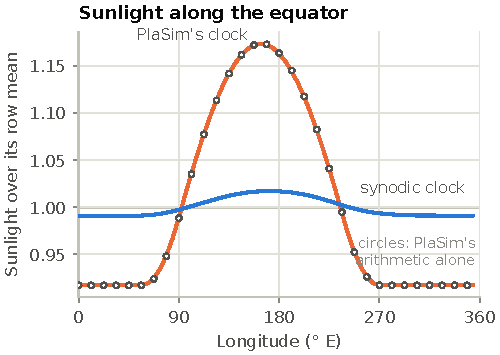
\includegraphics[width=0.6\textwidth]{figures/fig_sun_clock.pdf}
\caption{Sunlight at the top of the air along the equator, by longitude, over its row mean. Under PlaSim's
own Sun clock (the pre-correction run of Table~\ref{tab:states}, years 15--24) the Sun sweeps
392.5\textdegree\ each model day and skips back 32.5\textdegree, leaving 270--57\textdegree~E 8.3\% short
and the far side up to 17\% over; the circles rebuild that pattern from PlaSim's solar-position arithmetic
alone. Under the synodic clock, in a test from the same state, the row varies only by the 0.991--1.017 that
12.1 lunar days in a model year give.}
\label{fig:sunclock}
\end{figure}

\begin{table}[p]
\caption{Earth values and defects on the paths the lunar runs use. Form: a constant, a unit of time,
geometry, or a fit or simplification used beyond its range (Fit). Kind: a limitation (L) or a defect (D).
Repair: general; a general method with a lunar table; a calibration to the lunar design case; a setting of
the scenario; a capability added; a bound; a mitigation; avoided by configuration; bypassed; or open.
Opt-in repairs are off in the design case. The switches and lunar settings are in Table~\ref{tab:repairs}.}
\label{tab:inventory}
\footnotesize
\setlength{\tabcolsep}{3.5pt}
\renewcommand{\arraystretch}{1.08}
\begin{tabularx}{\textwidth}{@{}>{\raggedright\arraybackslash}p{0.13\textwidth}LL>{\raggedright\arraybackslash}p{0.083\textwidth}>{\centering\arraybackslash}p{0.04\textwidth}>{\raggedright\arraybackslash}p{0.12\textwidth}@{}}
\toprule
Part & Earth in the code & On the Moon & Form & Kind & Repair \\
\midrule
\multicolumn{6}{@{}l}{\textit{ExoPlaSim 3.4.2 (PlaSim)}} \\
Sun clock & Restarts each model day & Skips back 32.5\textdegree\ a day & Time & D & General \\
Convective cover & Rain converted per model day & Cover $+0.42$ & Time & D & General \\
Orbit default & Earth's orbit for 1~AD & Tilt 23.7\textdegree\ for 1.54\textdegree & Constant & D & General \\
Calendar & 360-day year of 17,280 steps & Output slips 120 steps a year & Time & L & General \\
Cloud water & CCM3 height scale in metres & Cloud above 20~km nearly dry & Constant & L & General \\
Vertical grid & Earth's $\sigma$ levels & Top layers above 63~km; two in the lowest 6.5~km & Geometry & L & Open \\
Slant path & Horizon factor 35 & 13.5 for water, 7.1 for air & Geometry & L & Method, lunar table \\
Columns & Flat, lit with the Sun up & Miss a net 5.8~W\,m$^{-2}$ loss & Geometry & L & Method, lunar table \\
Dynamics & Constant $g$, thin shell & $g$ 5.4\% lower at 48.6~km & Geometry & L & Open \\
Shortwave gases & Omit CO$_2$ and O$_2$ & Their share taken by water & Fit & L & Calibration \\
Rayleigh, continuum & 5772~K normalisation; continuum 0.024 & First design run past 310~K & Fit & L & Calibration \\
Water absorptivity & Lacis--Hansen, Earth's paths & Air 7.7--8.2 points short & Fit & L & Calibration \\
Longwave by height & Sasamori's absorptivities & Lowest layers overcooled 10--12~W\,m$^{-2}$ & Fit & L & Calibration, opt-in \\
Cloud phase & Liquid optics for all cloud & High cloud at 165--217~K reflects as liquid & Fit & L & General, opt-in \\
Saturation & Over liquid at every temperature & Cloud at 136--149\% of ice saturation & Fit & L & Open \\
Lowest level & Cause uncertain, probably the spectral transform & Up to 20~K cold in 0.8\% of windows & --- & ? & Open, screened \\
\midrule
\multicolumn{6}{@{}l}{\textit{CM1 release 22}} \\
Gravity & 9.81 in four routines on the lunar paths; fall speeds & Fall speeds 2.3--6 times too fast & Constant & L & General \\
Rain size & Mean under 2.8~mm; breakup from 0.3~mm & Stable drops 2.46 times larger & Fit & L & Open \\
RRTMG gases & CO$_2$ by year; Earth's trace gases & Earth's air & Constant & L & Setting \\
RRTMG pressures & Tables from 1,053.63~hPa & Lowest 7.5~km extrapolated & Fit & L & Open \\
RRTMG ice & Optics to 140~\textmu m & Run stopped at day 6.45 & Fit & L & Mitigation \\
RRTMG Sun & Unfiltered spectrum & 5~W\,m$^{-2}$ of clear-air absorption & Constant & L & Open \\
Sun and soil & Earth's day, calendar and tilt; soil 1--16~cm & Thermal wave 0.6~m deep & Time & L & General \\
Damping, mixing length & 300~s; 75~m & Earth's scales & Constant & L & General \\
Beta plane & Earth's rotation and radius & Earth's $\beta$ & Constant & L & Bypassed \\
Threads & Unlocated race & Runs on several threads part & --- & D & Open \\
\midrule
\multicolumn{6}{@{}l}{\textit{WRF-ELEC, grafted into CM1}} \\
Gravity, ventilation & 9.8; fall speeds; ventilation & Rain evaporates 1.3--1.5 times too fast if scaled alone & Constant & L & General \\
Breakdown cap & 180~kV\,m$^{-1}$ & Binds below 36~km & Constant & L & General \\
Ground strike & $-7$\,\textdegree C level; stopping field 0.15 & Level 27--34~km up & Constant & L & Bound \\
Sub-step & 0.75~s for 500~m layers & 2~km layers, slow graupel & Constant & L & General \\
Flash reach & Logged above a charge threshold & Weak high flashes logged none & Constant & L & General (logging) \\
Conduction & None in clear air & Charge persists for weeks & Time & L & Capability \\
Charging, thresholds & Laboratory laws; 50~MV, 10~kV\,m$^{-1}$ & Polarity turns with the law & Fit & L & Open \\
\midrule
\multicolumn{6}{@{}l}{\textit{SWAN 41.51 and SWASH 12.01}} \\
Wind-input knee & 1~Hz & Similarity off by 5.44\% & Constant & L & General \\
Air density & 1.28~kg\,m$^{-3}$ & About 1.40~kg\,m$^{-3}$ & Constant & L & Setting \\
Breaker parameter & Read uninitialised with breaking off & Repeats differ by 2.5\% & --- & D & Avoided \\
Unselected options & 2~s initial period; $g$ in ST6 and exact transfer; SWASH's rotation & Unused in the lunar runs & Constant & L & Avoided \\
Empirical laws & Wu, Komen, AGROW, breaker 0.73, breaking 0.6 and 0.3 & Uncalibrated & Fit & L & Open \\
\bottomrule
\end{tabularx}
\end{table}
